\documentclass[a4paper,9pt]{extarticle}

%=========================================================
% PACKAGES
%=========================================================

\usepackage[
a4paper,
top=1.8cm,
bottom=1.5cm,
footskip=7mm,
left=1cm,
right=1cm,
headheight=14pt,
headsep=5mm
]{geometry}
\usepackage[T1]{fontenc}
\usepackage[utf8]{inputenc}
\usepackage[french]{babel}

\usepackage[sfdefault]{FiraSans}
\renewcommand{\familydefault}{\sfdefault}

\usepackage{multicol}
\setlength{\columnsep}{0.7cm}

\usepackage{amsmath,amssymb}

\usepackage{titlesec}
\usepackage{enumitem}

\usepackage{tcolorbox}
\tcbuselibrary{skins,breakable}

\usepackage{xcolor}

\usepackage{graphicx}
\usepackage{float}

\usepackage{tikz}

\usepackage{fancyhdr}
\usepackage[hidelinks]{hyperref}


%=========================================================
% PAGE SETTINGS
%=========================================================

\setlength{\parindent}{0pt}
\setlength{\parskip}{1.5pt}

\setlength{\abovedisplayskip}{4pt}
\setlength{\belowdisplayskip}{4pt}

\setlist[itemize]{
leftmargin=*,
itemsep=1pt,
topsep=1pt
}


%=========================================================
% COLORS
%=========================================================

\definecolor{Blue}{HTML}{E3F0FF}
\definecolor{Green}{HTML}{E3F7EA}
\definecolor{Pink}{HTML}{FFE5ED}
\definecolor{Orange}{HTML}{FFF0DC}
\definecolor{Purple}{HTML}{EEE7FF}
\definecolor{Yellow}{HTML}{FFFADB}


\definecolor{BlueTitle}{HTML}{285B8F}
\definecolor{GreenTitle}{HTML}{287052}
\definecolor{PinkTitle}{HTML}{A84063}
\definecolor{OrangeTitle}{HTML}{A96500}
\definecolor{PurpleTitle}{HTML}{6245A5}


%=========================================================
% HEADER
%=========================================================

\pagestyle{fancy}

\fancyhf{}

\fancyhead[L]{\small\textbf{Game Theory and Strategic Decisions}}
\fancyhead[C]{\small Auctions: Private and Common Values}
\fancyhead[R]{\small Week 08 --- 02-08/11/2026}

\fancyfoot[C]{\small\href{https://github.com/AlphaXT38G/notes_ba5}{github.com/AlphaXT38G/notes\_ba5}}
\fancyfoot[R]{\small \thepage}

\renewcommand{\headrulewidth}{0.4pt}



%=========================================================
% TITLES
%=========================================================

\titleformat{\section}
{\large\bfseries\color{BlueTitle}}
{}{0pt}{}

\titlespacing{\section}
{0pt}{6pt}{3pt}


% separator

\newcommand{\separator}{
\vspace{2pt}
\hrule
\vspace{3pt}
}


%=========================================================
% BOXES
%=========================================================

% Boxes are kept whole (unbreakable): inside multicols, a box split by tcolorbox
% leaves an empty column behind it.

% DEFINITION - blue
\newtcolorbox{definition}{
enhanced,
unbreakable,
colback=Blue,
colframe=BlueTitle,
boxrule=0.7pt,
arc=0mm,
title=\textbf{Definition},
fonttitle=\bfseries
}

% IMPORTANT - pink
\newtcolorbox{important}{
enhanced,
unbreakable,
colback=Pink,
colframe=PinkTitle,
boxrule=0.7pt,
arc=0mm,
title=\textbf{Key idea},
fonttitle=\bfseries
}

% FORMULAS - green
\newtcolorbox{formula}{
enhanced,
unbreakable,
colback=Green,
colframe=GreenTitle,
boxrule=0.7pt,
arc=0mm,
title=\textbf{Key formulas},
fonttitle=\bfseries
}

% WARNING - orange
\newtcolorbox{warning}{
enhanced,
unbreakable,
colback=Orange,
colframe=OrangeTitle,
boxrule=0.7pt,
arc=0mm,
title=\textbf{Warning},
fonttitle=\bfseries
}

% EXAMPLE - purple
\newtcolorbox{example}{
enhanced,
unbreakable,
colback=Purple,
colframe=PurpleTitle,
boxrule=0.7pt,
arc=0mm,
title=\textbf{Example},
fonttitle=\bfseries
}

% SUMMARY - orange
\newtcolorbox{summary}{
enhanced,
unbreakable,
colback=Yellow,
colframe=OrangeTitle,
boxrule=0.7pt,
arc=0mm,
title=\textbf{Summary},
fonttitle=\bfseries
}



%=========================================================
% FIGURE BOX
%=========================================================

\newtcolorbox{figurebox}{
enhanced,
colback=white,
colframe=gray,
boxrule=0.5pt,
arc=0mm,
center
}



%=========================================================
% DOCUMENT
%=========================================================

\begin{document}

%\footnotesize   --> To reduce the size of the text

\thispagestyle{fancy}



\begin{multicols}{2}



%=========================================================
\section{This Week's Plan}


\begin{itemize}

\item Second part of the course: \textbf{auctions} (W.\ Vickrey, Nobel Prize 1996;
P.\ Milgrom, Nobel Prize 2020).

\item Types of auctions; private-value vs common-value auctions.

\item Optimal bids in \textbf{first-price} and \textbf{second-price} private-value auctions.

\item Common-value auctions and the \textbf{winner's curse}.

\end{itemize}


\begin{important}

An auction is a \textbf{Bayesian game} (Lectures 4--5): each bidder knows her own value (her
type), not the others'. A strategy is a bid for each value, $b(v)$.

\end{important}



%=========================================================
\section{Why Auctions?}


\begin{itemize}

\item \textbf{Price discovery}: for rare or unique objects (art works, historical
manufacts\dots) the price is whatever people are willing to pay.

\item \textbf{Efficiency of allocation}: especially for government auctions (spectrum rights,
carbon rights\dots): the business willing to pay more is likely the most productive one, the
one that gets the biggest benefit from the object.

\end{itemize}



%=========================================================
\section{Types of Auctions}


\begin{definition}

\textbf{OPEN AUCTIONS}

\begin{itemize}

\item \textbf{English}: ascending price (Christie's, Sotheby's).

\item \textbf{Dutch}: descending price (flower trading in Holland).

\end{itemize}

\textbf{SEALED-BID AUCTIONS}

\begin{itemize}

\item \textbf{First-price}: the highest bidder gets the object and pays \textbf{the price she
bid}. Equivalent to the Dutch auction.

\item \textbf{Second-price}: the highest bidder gets the object and pays \textbf{the price
bid by the second-highest bidder}. Equivalent to the English auction when the price ascends
continuously.

\end{itemize}

\end{definition}


\begin{important}

\textbf{Dutch $\equiv$ first-price}: you decide in advance where to stop the clock, learn
nothing before (when someone stops, it's over), and pay that price.

\textbf{English $\equiv$ second-price}: each bidder drops out when the price rises above her
value; just above the second-highest value, only the highest-value bidder remains and pays
(just above) the second-highest value.

\end{important}



%=========================================================
\section{Private vs Common Value}


\begin{definition}

Not about the format, but about the \textbf{object}.

\begin{itemize}

\item \textbf{Private value}: a different value $v_1, \ldots, v_N$ for each bidder, no
uncertainty about the object (quality, authenticity). Ex: last seat on a flight to Paris.

\item \textbf{Common value}: same value for all, but uncertain; each bidder has an imperfect
estimate (``signal''). Ex: an oil field. \textbf{Other people's estimates might change my
own.}

\end{itemize}

Many objects combine both: the guitar of Elvis Presley (authentic? and what is it worth?).

\end{definition}



%=========================================================
\section{Private-Value, First-Price Auction}


\begin{formula}

$N$ bidders; bidder $i$ knows her value $v_i$, not the others'. She bids $b(v_i)$. Payout:

\[
\mathcal{P}_i = (v_i - b_i)\; P(b_i > b_j \ \forall j \neq i)
\]

\end{formula}


Bidding $b_i = v_i$ gives 0 for sure, so bid $b_i < v_i$. \textbf{Two opposite forces}: a
higher $b_i$ gives a higher chance to win, but a lower ``surplus'' $v_i - b_i$.


\begin{center}

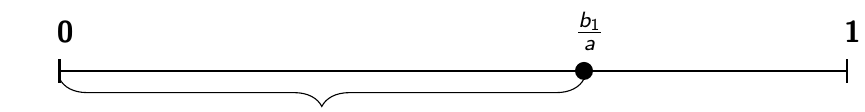
\includegraphics[
width=0.9\linewidth
]{../images/week08_01.png}

\end{center}


\begin{example}

\textbf{Two bidders, $v_i$ uniform on $[0,1]$}

Assume $b_2(v_2) = a v_2$. Bidder 1 wins if $v_2 < b_1/a$: probability $b_1/a$.

\[
\mathcal{P}_1 = (v_1 - b_1)\frac{b_1}{a}
\quad \Rightarrow \quad
\frac{v_1 - 2b_1}{a} = 0
\quad \Rightarrow \quad
b_1 = \frac{v_1}{2}
\]

Same for bidder 2: \textbf{BNE $b(v) = v/2$}.

\end{example}


\begin{definition}

\textbf{BID SHADING}: bidding less than the valuation of the object.

\end{definition}


\begin{formula}

\textbf{$N$ bidders}: $b_j = a_j v_j$. The events $b_j < b_1$ are independent, so

\[
P(b_j < b_1 \ \forall j) = \frac{b_1^{N-1}}{\prod_{j>1} a_j}, \qquad
\mathcal{P}_1 = (v_1 - b_1)\frac{b_1^{N-1}}{\prod_{j>1} a_j}
\]

Derivative: $-b_1^{N-1} + (N-1)(v_1 - b_1)b_1^{N-2} = 0$:

\[
b(v) = \frac{N-1}{N}\, v
\]

\end{formula}


\begin{example}

(Not on the slides) $v = 0.8$: $N = 2 \rightarrow 0.4$; $N = 5 \rightarrow 0.64$;
$N = 100 \rightarrow 0.792$. More competitors, less shading.

\end{example}



%=========================================================
\section{Private-Value, Second-Price Auction}


\begin{important}

\textbf{Bidding $b_i(v_i) = v_i$ is a (weakly) dominant strategy.} Most efficient
allocation; no knowledge about the other players (number, distribution of values) is needed.

\end{important}


\begin{formula}

\[
\text{payout} =
\begin{cases}
v_i - \max_{j \neq i} b_j & \text{if } b_i > \max_{j \neq i} b_j \\
0 & \text{otherwise}
\end{cases}
\]

The bid decides \emph{whether} you win, not \emph{what} you pay.

\end{formula}


\textbf{Overbidding} ($b_i > v_i$). Green: $v_i$, black: $b_i$, red: $\max_{j \neq i} b_j$.


\begin{itemize}

\item $\max b_j > b_i$: loses either way (payout 0).

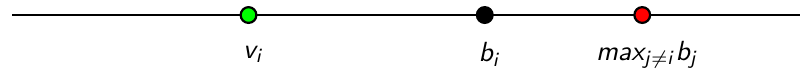
\includegraphics[width=0.9\linewidth]{../images/week08_02.png}

\item $v_i < \max b_j < b_i$: wins with a \textbf{negative payout}; bidding $v_i$ she'd lose
with 0. \textbf{Truthful is better.}

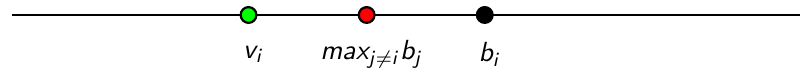
\includegraphics[width=0.9\linewidth]{../images/week08_03.png}

\item $\max b_j < v_i$: wins either way, same price.

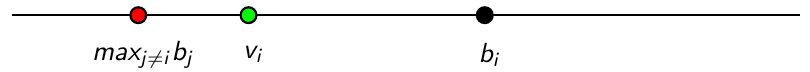
\includegraphics[width=0.9\linewidth]{../images/week08_04.png}

\end{itemize}


\textbf{Underbidding} ($b_i < v_i$):


\begin{itemize}

\item $\max b_j > v_i$: loses either way.

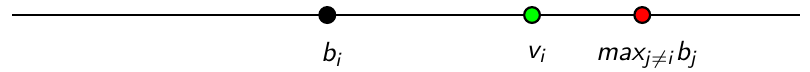
\includegraphics[width=0.9\linewidth]{../images/week08_05.png}

\item $b_i < \max b_j < v_i$: loses, but bidding $v_i$ she'd win with a \textbf{positive
payout}. \textbf{Truthful is better.}

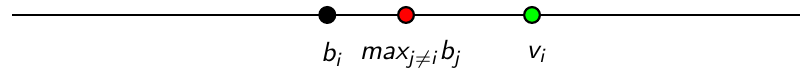
\includegraphics[width=0.9\linewidth]{../images/week08_06.png}

\item $\max b_j < b_i$: wins either way, same payout.

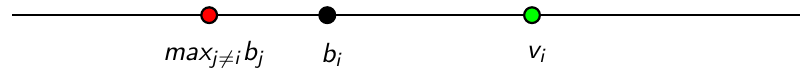
\includegraphics[width=0.9\linewidth]{../images/week08_07.png}

\end{itemize}



%=========================================================
\section{First-Price vs Second-Price}





\end{multicols}


\end{document}
